% !TeX document-id = {9f30a0a7-fd28-429c-b30f-1f1ceab3f7e5}
% tell Tex Studio to compile with --shell-escape to visualize SVGs
% !TeX TXS-program:compile = txs:///pdflatex/[--shell-escape]

\pdfsuppresswarningpagegroup=1

%\documentclass[11pt, a4paper, twoside=true, ngerman, parskip=full, listof=totoc,footsepline]{scrartcl} 
\documentclass[
11pt, 
a4paper, 
twoside=true, 
ngerman, 
parskip=full, 
listof=totoc, 
numbers=noenddot,
toc = bibnumbered	
]{scrartcl} 

% geschwungene Klammer Pflicht
% eckige Klammer optionaler Parameter
% article book report letter
% scrartcl scrreprt scrbook scrlettr2

% listof totoc alle Verzeichnisse werden ins Inhaltsverzeichnis aufgenommen

% standardpakete die immer sinnvoll sind
\usepackage[utf8]{inputenc}
\usepackage[ngerman]{babel}
\usepackage{csquotes}
% Schriftart wechseln
% LateX font catalogue
% use arial like clon
%\usepackage{arev}
%\usepackage[T1]{fontenc}

% Benutzen für Einheiten
\usepackage{siunitx}
\sisetup{locale=DE, per-mode=fraction, separate-uncertainty}

\usepackage{graphicx,amsmath,amssymb,amsfonts}

% nutze verbesserte schriftart von lateX
\usepackage{microtype}

% blindtext
\usepackage{blindtext}

% svg graphics
\usepackage[inkscapearea=page]{svg}

% microtype verbessert den Blocksatz
\usepackage{microtype}


% Ränder konfigurieren
\usepackage[left=3cm,right=3cm,top=2cm,bottom=2.5cm]{geometry}

% empty = keine Seitenzahl kein nichts
\pagestyle{empty}

% plain = nur seitenzahl
\pagestyle{plain}

\usepackage{scrlayer-scrpage}
\pagestyle{scrheadings}

\newcommand{\lka}{Landeskriminalamt SH}

% command für Vergleiche.
\newcommand{\vgl}[2]{\autocite[Vgl.][S.~2]{#1}}
% Nutzung \vgl{Literatur-ID}{Seitenangabe}

% command to bold and kursive
\newcommand{\boldIt}[1]{\textbf{\textit{#1}}}

% eine neue Environment erstellen
\newenvironment{beispiel}{\begin{center}\itshape\bfseries}{\end{center}}

%\automark{chapter}
\ihead[]{\headmark}
\chead[]{Benjamin Puhani}
\ohead[\today]{\today}
\cfoot[\lka]{\lka}
\ofoot[\pagemark]{\pagemark}


% Zeilenabstand ändern
%\usepackage[doublespacing]{setspace}
\usepackage[onehalfspacing]{setspace}

\doublespacing
\onehalfspacing


% Erstelle ein neues Inhaltsverzeichnis für Gleichungen
\DeclareNewTOC[type=equation,types=equations,listname={Gleichungsverzeichnis}]{equ}

% Erstelle Befehl um eine Neue Equation dem Verzeichnis hinzuzufügen
\newcommand{\myequations}[1]{\addcontentsline{equ}{equation}{\protect\numberline{\theequation}~~#1}}

\usepackage{newfloat}
\DeclareFloatingEnvironment[fileext=loa, name=Gleichung]{gleichung}

% Erstelle einen Math operator
\DeclareMathOperator{\sincos}{}

% Tabellen mit booktabs
% \toprule
% \midrule
% \bottomrule
\usepackage{booktabs}

% verwendet für die zitation
\usepackage[backend=biber,style=ieee,bibwarn=true,bibencoding=utf8]{biblatex}
% bibdatei hinzufügen
\addbibresource{bibliography/literature.bib}

%\usepackage{pgfplot}

% muss als vorletztes Paket geladen werden
\usepackage[]{hyperref}

% Paket für Referencen
% muss letzter Import eines Paketes sein.
% Erkennt was es ist und ist besser als normales LateX
\usepackage[noabbrev]{cleveref}

% Auskommentieren mit Strg + T


\begin{document}
	
	\begin{titlepage}
	\begin{center}
		\begin{figure}
			\centering
			\includesvg[width=7cm]{images/fachhochschule-kiel-logo.svg}
		\end{figure}
		Fachhochschule Kiel\\
		Fachbereich Informatik und Elektrotechnik\\
		Studiengang Informatik (B.Sc)\\
		Maschinelles Lernen\\
		Herr Prof. Dr. Patrick Hennig\\
		WiSe 2024/25\\
		
	\end{center}
	\vfill
	\begin{center}
		\Huge \textsc{\mytitle}
		
		
		\vfill
		
		\LARGE
		Hausarbeit
		
		\vspace{1cm}
		vorgelegt von\\
		Benjamin Puhani\\
		Matr. Nr.: 941077\\
		am \today{}
	\end{center}
	\vfill
	
	
	\begin{tabular}{@{}l@{\hspace{2cm}}l@{}}
		Erstprüfer:   & Herr Prof. Dr. Patrick Hennig\\
	\end{tabular}

\end{titlepage}



%Titel der Arbeit,
%Zweck der Arbeit (Thesis zur Erlangung des Grades Bachelor / Master of Science /
%Engineering),
%Organisation (Fachhochschule Kiel, Fachbereich Informatik und Elektrotechnik),
%Autor (euer Name),
%Abgabedatum,
%Matrikelnummer,
%Namen von Erst- und Zweitprüfer,
%ggf. Name des Betreuers in der Firma,
%ggf. Name und Anschrift der Firma,
%evtl. das Logo der FH-Kiel
	
	\begin{abstract}
Diese Arbeit entstand als Antwort auf die spezifische Aufgabenstellung, mindestens zwei Klassifikationsmethoden auf einen Datensatz anzuwenden, der mindestens 200 Elemente umfasst, Klassen aufweist, die nicht linear separierbar sind, und einen Merkmalsraum mit mindestens zwei Dimensionen besitzt. In dieser Studie wurden das k-Nächster-Nachbarn (k-NN)-Verfahren und Support-Vektor-Maschinen (SVM) zur Klassifikation zweier Pistazienarten verwendet. Die Untersuchung folgte einem strukturierten Ansatz, der eine explorative Datenanalyse, Datenbereinigung, Aufteilung in Trainings- und Testdaten, eine systematische Variation von Hyperparametern sowie deren Bewertung mit geeigneten Qualitätsmaßen umfasste. Die signifikante Verbesserung der Klassifikationsgenauigkeit durch Hyperparameter-Optimierung und Merkmalsnormalisierung demonstriert die Effektivität beider Methoden in diesem spezifischen Anwendungsfeld. Besondere Aufmerksamkeit wurde dem Einfluss von Hyperparametereinstellungen auf die Leistungsfähigkeit der Modelle gewidmet, wobei für k-NN durch die Variation des 'k'-Wertes und die Auswahl von sechs Merkmalen eine optimale Genauigkeit von 89,64 \% erreicht wurde. Im Vergleich dazu wurde durch die Anwendung eines systematischen \glqq{}GridSearch\grqq{}-Verfahrens zur Optimierung der Hyperparameter für SVM eine ähnlich hohe Leistung erzielt.
Die Ergebnisse bieten Einblicke in die Potenziale und Herausforderungen bei der Anwendung von k-NN und SVM in der nicht-linearen Klassifikation und unterstreichen die Bedeutung sorgfältiger Datenanalyse und -aufbereitung für die Modellgenauigkeit. Zukünftige Forschungen könnten sich auf die Vertiefung der Untersuchung von Overfitting konzentrieren, um die Generalisierbarkeit der Modelle zu verbessern. 

%Diese Studie bietet einen Überblick über die Anwendung des k-NN-Verfahrens zur Klassifikation von Daten unter besonderer Berücksichtigung von Skalierungs- und Normalisierungstechniken.
%Aufgrund des begrenzten Umfangs dieser Arbeit werden detaillierte Analysen, einschließlich umfassender Datenvisualisierungen und Codebeispiele, in einem ergänzenden Jupyter Notebook bereitgestellt, das für eine vertiefte Betrachtung herangezogen werden kann.
\end{abstract}

	
	\pagenumbering{Roman}
	\cleardoublepage % Stellt sicher, dass das TOC auf einer neuen Seite beginnt
	\phantomsection
	\hypertarget{toc}{}
	\tableofcontents
	\listoffigures
	\listoftables
	
	
\section{Einleitung}

- Hier wird das Thema eingeführt, die Problemstellung erläutert 
- Zielsetzung der Arbeit wird hier klar formuliert

- Zudem wird i. d. R. der Aufbau der Arbeit kurz umrissen.
Auch hier schon passive Formulierungen:
- „…


In dieser Arbeit wird die Anwendung von K-Nächster-Nachbarn (K-NN)-Verfahren und Support-Vektor-Maschinen (SVM) für die Klassifizierung zweier Pistazienarten untersucht. 

% Zielsetzung
Ziel ist es den Einfluss an Hyperparametern 

% Aufbau der Arbeit
\subsection{Aufbau}
Zunächst wird der vorliegende Datensatz eingeführt, genauer analysiert, aufbereitet und in Trainings- sowie Testdaten aufgeteilt.
Sobald der Datensatz gründlich vorbereitet wurde wird mit der Klassifikation mittels K-NN Verfahren begonnen. 
Es wird mit unterschiedlichen \glqq{}K\grqq{} und Anzahl an Attributen trainiert. 
Die Ergebnisse werden unter anderem auf Genauigkeit und F1-Score anhand der Testdaten mit einander verglichen.
Anschließend werden SVMs als Klassifizierungswerkzeug benutzt. Und ähnlich wie beim K-NN Verfahren versucht optimale Hyperparameter zu finden.




1. Klassifikation mit K-NN
verfügbare Hyperparameter:
 k - Die Anzahl an zu betrachtenden Nachbarn
 attribute - 16 zur Verfügung stehende
Es wurde eine Klasse erstellt welche es erleichtert verschiedene Kombinationen an Attributen und Ks auf ihre Genauigkeit zu testen. 

	\section{Daten und Methoden}

In dieser Arbeit wird ein Datensatz verwendet, der im Rahmen der Publikation "Progress of Nutrition Vol. 23 No. 2 (2021)" veröffentlicht und in der Studie "Classification of Pistachio Species Using Improved k-NN Classifier"\cite{Ozkan.2021} vorgestellt wurde. Der Datensatz ist öffentlich zugänglich und speziell für die Klassifikation zweier Pistazienarten (\glqq{}Kirmizi\grqq{} und \glqq{}Siirt\grqq{}) erstellt worden. Für diese Studie wurden 2148 hochauflösende Bilder von diesen zwei Pistazienarten aufgenommen. Anhand dieser Aufnahmen konnten die Merkmale gemessen werden.

\subsection{Explorative Datenanalyse} 
Der Datensatz beinhaltet zwei Versionen mit einem unterschiedlichen Umfang an Merkmalen: eine Version umfasst 16 Features, während die andere Version 28 Features bietet. Für die Zwecke dieses Projekts wird die Version mit 16 Features verwendet. Die Auswahl dieser Version erfolgte aufgrund der Tatsache, dass die zusätzlichen 12 Features Farbmerkmale der Pistazien darstellen, welche in dieser spezifischen Arbeit nicht berücksichtigt werden.

Die für dieses Projekt verwendeten Merkmale lassen sich in die folgenden Kategorien unterteilen:

\textbf{Morphologische Merkmale (12 Features):}
\begin{itemize}[itemsep=0pt, parsep=0pt]
	\item Fläche (Area)
	\item Umfang (Perimeter)
	\item Hauptachse (Major\_Axis)
	\item Nebenachse (Minor\_Axis)
	\item Exzentrizität (Eccentricity)
	\item Äquivalentdurchmesser (Eqdiasq)
	\item Solidität (Solidity)
	\item Konvexe Fläche (Convex\_Area)
	\item Ausdehnung (Extent)
	\item Seitenverhältnis (Aspect\_Ratio)
	\item Rundheit (Roundness)
	\item Kompaktheit (Compactness)
\end{itemize}

\textbf{Formmerkmale (4 Features):}
\begin{itemize}[itemsep=0pt, parsep=0pt]
	\item Formfaktor 1 (Shapefactor\_1)
	\item Formfaktor 2 (Shapefactor\_2)
	\item Formfaktor 3 (Shapefactor\_3)
	\item Formfaktor 4 (Shapefactor\_4)
\end{itemize}

Die vier Formmerkmale sind weitere mathematische Zusammenfassungen zwischen einzelnen morphologischen Merkmalen.
Was sich genau hinter den Bezeichnungen versteckt lässt sich unter \parencite[4]{Ozkan.2021} in Tabelle 1 nachlesen.

%\textbf{Korrelation zwischen Merkmalen}\\
%Wie zu erwarten besteht zwischen mehreren Merkmalen eine hohe Abhängigkeit.
%Beispielsweise ist die Fläche sehr stark abhängig von der Haupt- und Nebenachse einer Pistazie.
%Visualisieren lässt sich das ganze mittels einer Korrelationsmatrix.
%
%\noindent\hspace*{-0.3cm}% Negative horizontale Verschiebung
%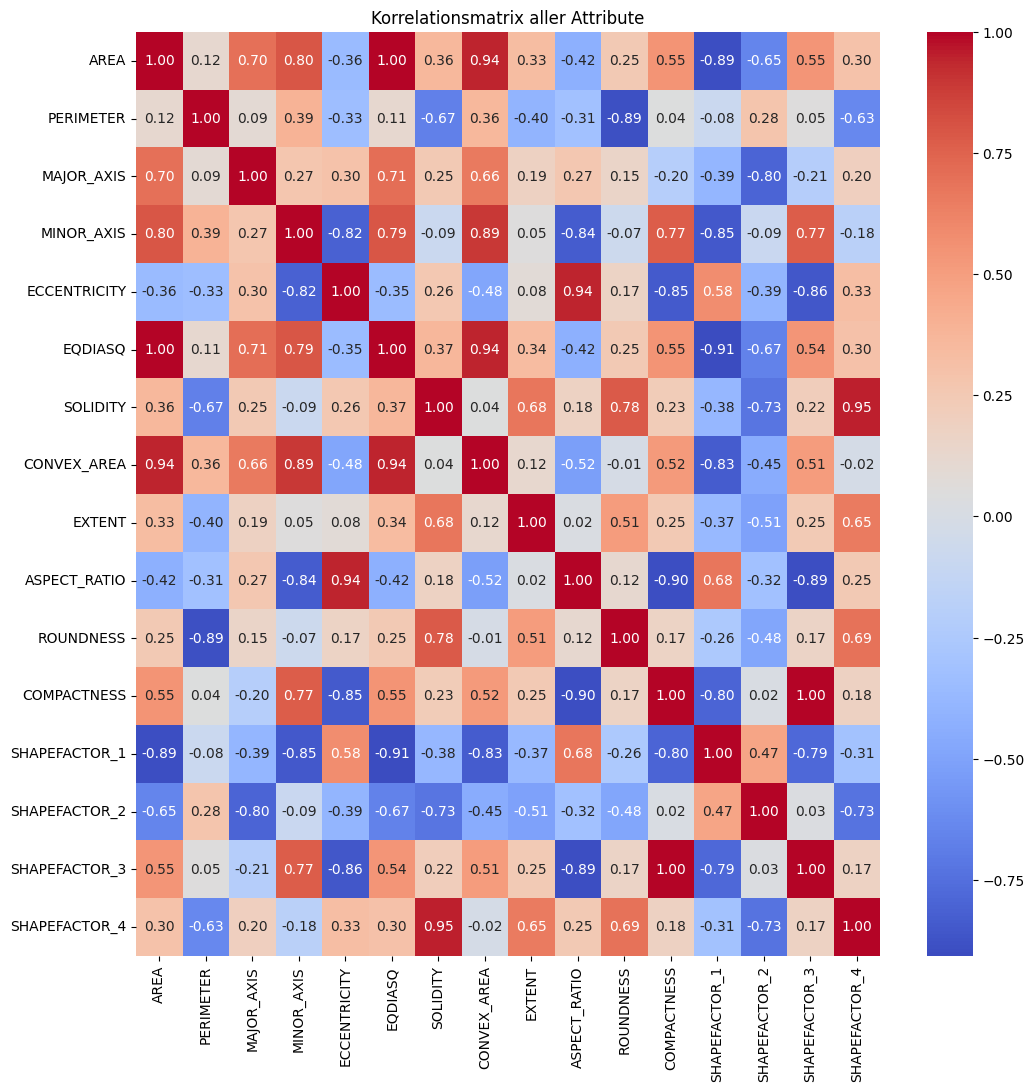
\includegraphics[width=1.1\linewidth]{images/korrelationsmatrix_aller_attribute}
%\captionof{figure}{Korrelationsmatrix der Pistazienmerkmale.}
%\label{fig:korrelation_of_attributes}
%
%
%Die Korrelationsmatrix in \autoref{fig:korrelation_of_attributes} bestätigt nicht nur die vermuteten Abhängigkeiten, wie der Fläche und den Achsen, sonder zeigt im Besonderen deutliche negative Korrelationen zwischen verschiedenen Formmerkmalen und den morphologischen Eigenschaften auf.

\textbf{Verteilung der Klassen}\\
Zum trainieren eines Klassifizierung Modells ist es wichtig, dass Klassen in den Trainingsdaten ausgewogen verteilt sind, da ansonsten Vorhersagemodelle dazu neigen können, die Klasse mit der höchsten Anzahl von Beobachtungen hervorzusagen ungeachtet der tatsächlichen Klasse \cite{ZoumanaKeita.2024}.

In dem vorliegenden Datensatz ist die Klasse der Kirmizi-Pistazien mit 1232 Einträgen, gegenüber den Siit-Pistazien mit 916 Einträgen deutlich überrepräsentiert, wie in \autoref{fig:distribution_of_classes} dargestellt.
Dies wird auch in dem \autoref{sec:aufteilung-in-trainings-und-testdaten} bei der Aufteilung in die Trainings- und Testdaten berücksichtigt.

{
	\centering
	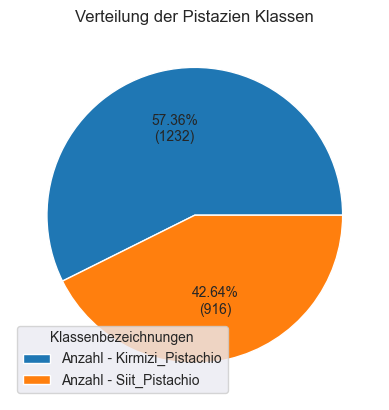
\includegraphics[width=1\linewidth]{images/distribution_of_classes}
	\captionof{figure}{Klassenverteilung innerhalb der 2148 Pistaziendatensätze.}
	\label{fig:distribution_of_classes}
}


\subsection{Bereinigung des Datensatzes}
\label{subsec:cleaning-the-data}
Der Datensatz wurde auf Null Werte und Duplikate überprüft. Es konnten keine gefunden werden.
Auch wurden die Daten in Bezug auf die einzelnen Zahlenbereiche der Merkmale untersucht. Diese liegen, wie \autoref{tab:deskriptive_statistik} zeigt, teilweise sehr weit auseinander.\\

{	
	\tiny
	\centering
	\begin{tabular}{lrrrr}
		\toprule
		{Merkmal} & {Mean} & {Std} & {Min} & {Max} \\
		\midrule
		AREA          & 79950.66 & 13121.74 & 29808 & 124008 \\
		PERIMETER     & 1425.97  & 375.57   & 858   & 2755 \\
		MAJOR\_AXIS    & 446.25   & 32.45    & 320   & 542 \\
		MINOR\_AXIS    & 238.31   & 30.31    & 134   & 383 \\
		ECCENTRICITY  & 0.84     & 0.05     & 0.50  & 0.95 \\
		EQDIASQ       & 317.92   & 26.91    & 195   & 397 \\
		SOLIDITY      & 0.94     & 0.05     & 0.59  & 1.00 \\
		CONVEX\_AREA   & 85015.84 & 13154.92 & 37935 & 132478 \\
		EXTENT        & 0.72     & 0.05     & 0.43  & 0.82 \\
		ASPECT\_RATIO  & 1.90     & 0.24     & 1.16  & 3.09 \\
		ROUNDNESS     & 0.57     & 0.21     & 0.06  & 0.93 \\
		COMPACTNESS   & 0.71     & 0.04     & 0.48  & 0.88 \\
		SHAPEFACTOR\_1 & 0.01     & 0.00     & 0.004 & 0.013 \\
		SHAPEFACTOR\_2 & 0.003    & 0.00034  & 0.002 & 0.005 \\
		SHAPEFACTOR\_3 & 0.51     & 0.06     & 0.23  & 0.77 \\
		SHAPEFACTOR\_4 & 0.96     & 0.05     & 0.62  & 1.00 \\
		\bottomrule
	\end{tabular}
	\captionof{table}{Übersicht der deskriptiven Statistik aller Merkmale}
	\label{tab:deskriptive_statistik}
}

Insbesondere weisen die erheblichen Unterschiede zwischen den maximalen und minimalen Werten einiger Merkmale, wie beispielhaft bei der konvexen Fläche (maximaler Wert: 132478) im Vergleich zum Formfaktor 2 (minimaler Wert: 0.002) dargestellt, auf eine breite Streuung innerhalb der Daten hin. Diese ausgeprägte Varianz in den Datengrößenordnungen kann beim k-NN Verfahren zu Herausforderungen führen, da k-NN auf Distanzmessungen basiert und somit ungleich gewichtete Merkmale zu verzerrten Ergebnissen führen können \cite{Lang.2023}. Die unterschiedlichen Größenordnungen bedeuten, dass Merkmale mit größeren numerischen Werten einen unverhältnismäßig hohen Einfluss auf die Distanzberechnung haben, was die Leistungsfähigkeit des Klassifikators beeinträchtigt.
Diese Beobachtung wird im \autoref{subsec:importance-of-normalizing} anhand eines direkten Vergleichs auf die Probe gestellt.

\textbf{Skalierung und Normalisierung}\\
Mittels Min-Max-Normalisierung wurden die Daten auf einen Bereich von [0,1] gebracht.
Durch die Anpassung aller Merkmale auf dieselbe Skala wird gewährleistet, dass jedes Attribut gleichberechtigt in die Berechnung der Distanzen eingeht.
Eine Übersicht der normalisierten Werte wird in \autoref{tab:normalisierte_deskriptive_statistik} dargestellt.\\

%#### Datenbereinigung
%1. Überprüfung auf und entfernen von Null-Werten
%2. Überprüfung auf und entfernen von Duplikaten
%3. Überprüfung der Zahlenbereiche
%4. Überprüfung der Größenverhältnisse der Klassen

{
	\tiny
	\centering
	\begin{tabular}{lrrrr}
		\toprule
		{Merkmal}        & {Mean}    & {Std}     & {Min} & {Max} \\
		\midrule
		AREA           & 0.5323  & 0.139297 & 0.0 & 1.0 \\
		PERIMETER      & 0.299263 & 0.198011 & 0.0 & 1.0 \\
		MAJOR\_AXIS     & 0.568106 & 0.146400 & 0.0 & 1.0 \\
		MINOR\_AXIS     & 0.419988 & 0.121468 & 0.0 & 1.0 \\
		ECCENTRICITY   & 0.760188 & 0.110539 & 0.0 & 1.0 \\
		EQDIASQ        & 0.607799 & 0.132855 & 0.0 & 1.0 \\
		SOLIDITY       & 0.864880 & 0.123931 & 0.0 & 1.0 \\
		CONVEX\_AREA    & 0.497983 & 0.139142 & 0.0 & 1.0 \\
		EXTENT         & 0.734656 & 0.133602 & 0.0 & 1.0 \\
		ASPECT\_RATIO   & 0.383777 & 0.124579 & 0.0 & 1.0 \\
		ROUNDNESS      & 0.581502 & 0.244327 & 0.0 & 1.0 \\
		COMPACTNESS    & 0.589890 & 0.110841 & 0.0 & 1.0 \\
		SHAPEFACTOR\_1  & 0.186951 & 0.089808 & 0.0 & 1.0 \\
		SHAPEFACTOR\_2  & 0.212820 & 0.117162 & 0.0 & 1.0 \\
		SHAPEFACTOR\_3  & 0.521804 & 0.117540 & 0.0 & 1.0 \\
		SHAPEFACTOR\_4  & 0.884413 & 0.136927 & 0.0 & 1.0 \\
		\bottomrule
	\end{tabular}
	\captionof{table}{Übersicht der normalisierten deskriptiven Statistik aller Merkmale}
	\label{tab:normalisierte_deskriptive_statistik}
}

\subsection{Aufteilung in Trainings- und Testdaten}
\label{sec:aufteilung-in-trainings-und-testdaten}

 Um sicherzustellen, dass das Modell gut generalisiert und nicht nur auf den ihm zur Trainingszeit präsentierten Daten funktioniert, wird für den Datensatz eine ausgewogene Datenaufteilung vorgenommen. Zunächst wird die Anzahl der Datensätze beider Klassen durch \grqq{}Resampling\glqq{} angeglichen, um einen ausgeglichenen Datensatz zu erhalten, der keine Verzerrung zugunsten einer Klasse aufweist. Anschließend werden die Daten in Features (die 16 Merkmale) und Labels (die Klasse der Pistazie) aufgeteilt. Der nächste Schritt teilt diese Daten in ein Trainingsset (80 \% der Daten) und ein Testset (20 \% der Daten). Hierbei wird sichergestellt, dass das Verhältnis der Klassen im Trainings- und im Testset dem des gesamten Datensatzes entspricht, was zur Validität des Lernverfahrens beiträgt. Mit dieser Methode wird sichergestellt, dass das jeweilige Modell auf einer soliden und repräsentativen Datenbasis trainiert und evaluiert wird.

\subsection{Methoden}

Für die Klassifikation zweier Pistazienarten auf Grundlage von 16 Merkmalen wurde sich für k-NN und SVM entschieden, wofür es mehrere Gründe gibt.

Zunächst bietet k-NN den Vorteil der Einfachheit und Anschaulichkeit. 
Er ist intuitiv nachvollziehbar und ermöglicht damit ein leichtes Verständnis der dahinterliegenden Mechanismen.
Die Effektivität von k-NN in Anwendungsszenarien, bei denen die Beziehungen zwischen Datenpunkten räumlich interpretierbar sind, macht ihn für das Klassifikationsproblem der Pistazienarten besonders geeignet.
Ein Nachteil dieses Verfahrens ist, dass es am \glqq{}Fluch der Dimensionalität\grqq{} leidet, dies bedeutet, dass je mehr Merkmale in einem Datenraum miteinander verglichen werden, desto mehr leidet die Modellgenauigkeit und -effizienz \cite{Lang.2023b}.

SVM sind hingegen darauf ausgelegt mit hohen Dimensionen umzugehen, indem eine Hyper-Ebene in einem hochdimensionalen Raum konstruiert wird\cite{Cortes.1995}. Dies macht SVM im Gegensatz zu k-NN extrem leistungsfähig, wenn es um einen Datensatz mit einer großen Anzahl an Merkmalen geht.

Durch die Benutzung von k-NN und SVM lassen sich die Stärken beider Algorithmen nutzen.\\

\textbf{K-NN}\\
Um ein besseres Verständnis über die Wichtigkeit der Skalierung zu gewinnen wurde, wie bereits in \autoref{subsec:cleaning-the-data} angedeutet, der Algorithmus mehrmals normalisiert und nicht normalisiert auf den Datensatz angewandt.
Weiterhin wurde, zur Verbesserung des k-NN Verfahrens, zum einen der Hyperparameter \glqq{}k\grqq{} kontinuierlich verändert.
Sowie aufgrund des \glqq{}Fluchs der Dimensionalität\grqq{} die Anzahl an Merkmalen auf denen der Algorithmus trainiert und getestet wird angepasst.

\begin{itemize}[itemsep=0pt, parsep=0pt]
	\item Für jeden Trainingsdurchlauf wurden 100 unterschiedliche \glqq{}k\grqq{} probiert.
	\item Es wurde jede mögliche Kombination der 16 Merkmale ausprobiert.
\end{itemize}
 
Wie viele unterschiedliche Kombinationen (ohne Reihenfolge) es gibt lässt sich mit der Binomial Formel in \autoref{fig:sum_binom_kombinations} ausrechnen.
Diese 65635 multipliziert mit den jeweils 100 k ergibt eine Summe von $6563500$ durchläufen des k-NN Verfahrens.
Es wurde immer das beste \glqq{}k\grqq{} in einer Tabelle gespeichert. Diese CSV-Datei \glqq{}data/knn\_all\_combinations.csv\grqq{} liegt dieser Arbeit bei.
\vspace{-10pt}
$$
\sum_{i=1}^{16} \binom{16}{i} = 65535
$$
\captionof{figure}{Summe aller möglichen Kombinationen von 16 Merkmalen}
\label{fig:sum_binom_kombinations}

\textbf{SVM}\\
Die Anpassung der Hyperparameter des SVM-Modells erfolgt mittels \glqq{}GridSearch\grqq{} einer Methode, die systematisch eine Reihe von vordefinierten Hyperparametern ausprobiert, um die beste Kombination für die Modellleistung zu finden.
In dieser Arbeit wurden der Regulierungsparameter \glqq{}C\grqq{}, der \glqq{}Gamma\grqq{}-Wert und der \glqq{}Kernel\grqq{}-Typ angepasst.
\autoref{fig:hyperparameter_svn} zeigt die Werte welche für die \glqq{}GridSearch\grqq{} benutzt wurden. 

%\vspace{-10pt} % Verringern des Raums vor der Verbatim-
\begin{verbatim}
'C': [0.1, 1, 10, 100],
'gamma': [1, 0.1, 0.01, 0.001],
'kernel': ['rbf', 'poly', 
  'sigmoid', 'linear']
\end{verbatim}
%\vspace{-10pt}
\captionof{figure}{SVM Hyperparameter}
\label{fig:hyperparameter_svn}


\section{Ergebnisse}\label{sec:Ergebnisse}
Alle Ergebnisse dieser Arbeit stammen aus dem anhängenden Jupyter Notebook \glqq{}ml\_bp\_pistachios.ipynb\grqq{} und können dort im Detail nachvollzogen werden. 

\subsection{Die Wichtigkeit der Normalisierung}
\label{subsec:importance-of-normalizing}

{
	\centering
	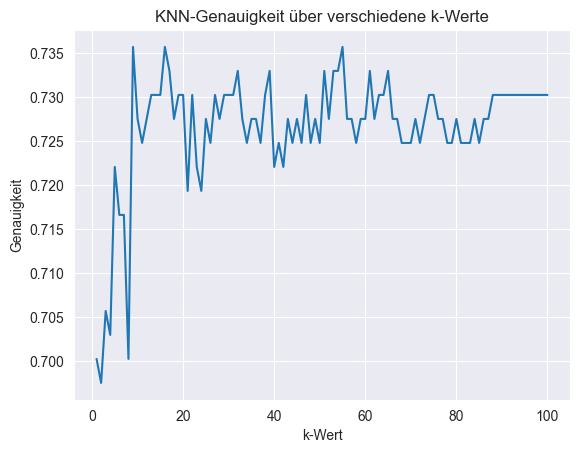
\includegraphics[width=0.9\linewidth]{images/knn_all_attributes}
	\captionof{figure}{Test-Genauigkeit bei 16 Merkmalen mit der Besten bei: 73,56 \%, F1-Score: 0.74 mit k: 9}
	\label{fig:knnallattributes}
}

{
	\centering
	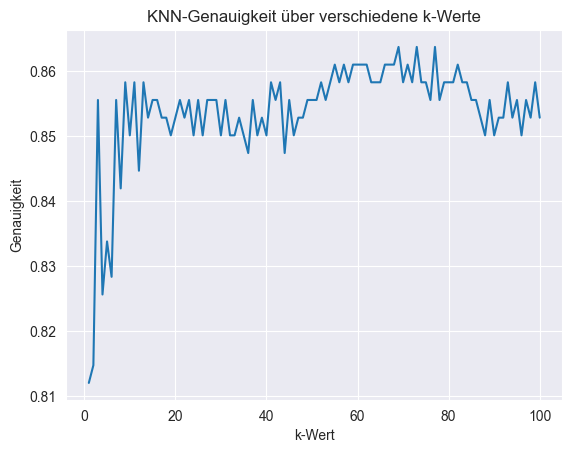
\includegraphics[width=0.9\linewidth]{images/knn_normalized_all_attributes}
	\captionof{figure}{Test-Genauigkeit bei 16 normalisierte Merkmalen mit der Besten bei: 86,37 \%, F1-Score: 0.86 mit k: 69}
	\label{fig:knnnormalizedallattributes}
}

Dabei zeigt sich in \autoref{fig:knnallattributes} im Vergleich zu \autoref{fig:knnnormalizedallattributes}, dass durch die Normalisierung eine deutliche Verbesserung (mehr als 10 \% Genauigkeit) der Klassifikationsergebnisse erzielt werden kann.
Alle anschließenden Operationen basieren auf einem normalisierten Datensatz.

\subsection{Parameter Optimierung bei K-NN}
{
	\centering
	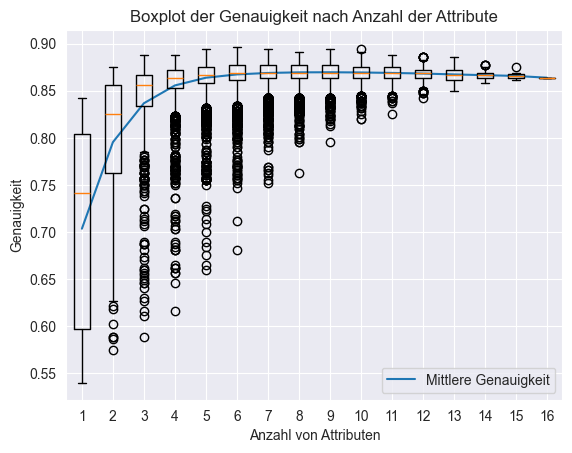
\includegraphics[width=1\linewidth]{images/best_knn_of_all_combinations}
	\captionof{figure}{Auswertung aller Kombinationen der 16 Merkmale}
	\label{fig:bestknnofallcombinations}
}

Das k-NN Modell welches am besten Abschnitt erzielte eine Test-Genauigkeit von 89,64 \%, F1-Score von: 0.90, auf Grundlage von: \glqq{}k\grqq{} = 39 mit den Merkmalen:
\begin{itemize}[itemsep=0pt, parsep=0pt]
	\item MAJOR\_AXIS
	\item EQDIASQ
	\item SOLIDITY
	\item EXTENT
	\item COMPACTNESS
	\item SHAPEFACTOR\_4
\end{itemize}

\subsection{Parameter Optimierung bei SVM}
{
	\centering
	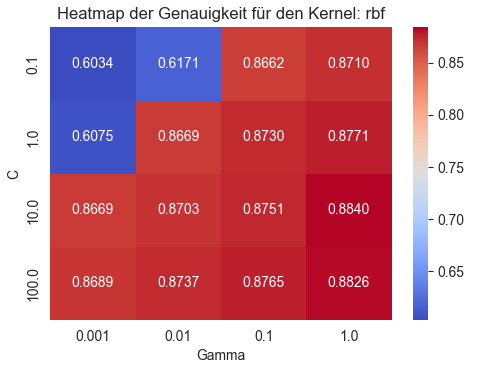
\includegraphics[width=1\linewidth]{images/svm_gridsearch_rbf}
	\captionof{figure}{GridSearch SVM Optimierung für rbf mit verschiedenen Hyperparametern}
	\label{fig:svmgridsearchrbf}
}
Die \glqq{}GridSearch\grqq{} liefert eine optimierte SVM mit den folgenden Hyperparameter zurück:
\begin{verbatim}
	C: 10; Gamma: 1; Kernel-Type: rbf
\end{verbatim}
 Dies geht auch aus \autoref{fig:svmgridsearchrbf} hervor. Für diese Konfiguration konnte ein F1-Score von 0.88 erreicht werden und eine Test-Genauigkeit von 87,73 \%.
 Die übrigen Heatmaps lieferten schlechtere Ergebnisse und sind hier aus Platzgründen entfernt worden.










	\section{Diskussion}

- Diskussion der Ergebnisse inkl. eines Vergleichs der Methoden
	
	
	\printbibliography[heading=bibintoc]
	\appendix\pagenumbering{roman}
	
	
\end{document}
